\section{Theory-Directed Simulation and Analysis}
\label{sec:evaluation}

\subsection{Validation design and execution models}
The experiments check predictions derived before each batch, rather
than tune gains to obtain a favorable comparison. We distinguish
the proof-matched continuous fluid reference from continuous-phase
Callisto. The reference uses the triangle, capacity $\beta_{\max}=2048$, gains
and physical period of Section~\ref{sec:btd_reference}, zero delays,
zero memory and compatible initial occupancy/target/marking $z$.
Fuzzy executes the original 25-rule implementation; its central
formula is used in the separate proof, not as the sole simulator.
The horizon is $T=2001H$, comprising the bootstrap and 2000 further
held-flow intervals. Full trajectories include every endpoint;
affine interpolation covers intersample extrema.

Validation comprises 34 new reference trajectories, six verified
cached sources and 12 new Callisto runs. The reference cases check
target translation, mismatch boundaries, equal-spread directions
and uniform-interval endpoints. These are qualitative consistency
checks informed by theory and earlier results. Proof computations
and translated maps are separate from plant runs; full protocols
and counts appear in Appendix~\ref{app:safety_validation}.

Callisto keeps continuous physical phase, integer frame events,
local polling $p=1000$, execution delay $d_{\rm ctrl}=10$ and constant
physical link latency 20. Initial phases are 0.1 and negative-time
history is preserved. Each case sets $\beta_e(0)=\beta_e^*=z$,
Fuzzy's percentage setpoint to $100z/\beta_{\max}$, and the marking to $z$ plus
the initial in-flight count. The two controllers share these values
and the uncontrolled frequency vector. Capacity and matched gains
remain fixed. Guards are enabled with zero reserve; observer,
supervisory switching and anti-windup are disabled. We record
complete-event buffer extrema, positive physical frequencies,
limiter use, guard-off episodes and data progress. A guard-supported
capacity invariant is distinguished from normal unstalled control.

Within each pair, capacity, compatible initialization, gain coordinates
and execution policies are shared; the control law is the variable.
Near-boundary targets test reserve requirements and are not proposed
replacements for half-capacity centering. Table~\ref{tab:safety_prediction_evidence}
maps each theoretical prediction to its verification and scope.

\subsection{Reference safety and mismatch--occupancy relation}
At $s=1$, direct runs use $z\in\{16,20,24,2024,2028,2032\}$.
The nonzero-target executions reproduce the proved translation
identity with maximum occupancy residual $6.83\times10^{-13}$ frame
and phase residual $2.78\times10^{-12}$. No comparison tolerance is
loosened. At $z=20$, Fuzzy's observed range is approximately
$[2.685943,37.314057]$, consistent with the certified all-time
interval $(2.685,37.315)$. PI's unprotected reference reaches
$-3.403701$ on a receiving channel. Both controllers cross at
$z=16$ and both remain strictly safe at $z=24$; the upper-target
mirror checks agree under the zero-delay reference assumptions.
Figure~\ref{fig:safety_reference_z20} shows the raw startup response.
Negative occupancy after the first crossing is a diagnostic virtual
continuation, never a physical buffer. The all-time conclusion comes
from the prefix/tail certificate, not the finite simulation horizon.

\begin{figure*}[t]
 \centering
 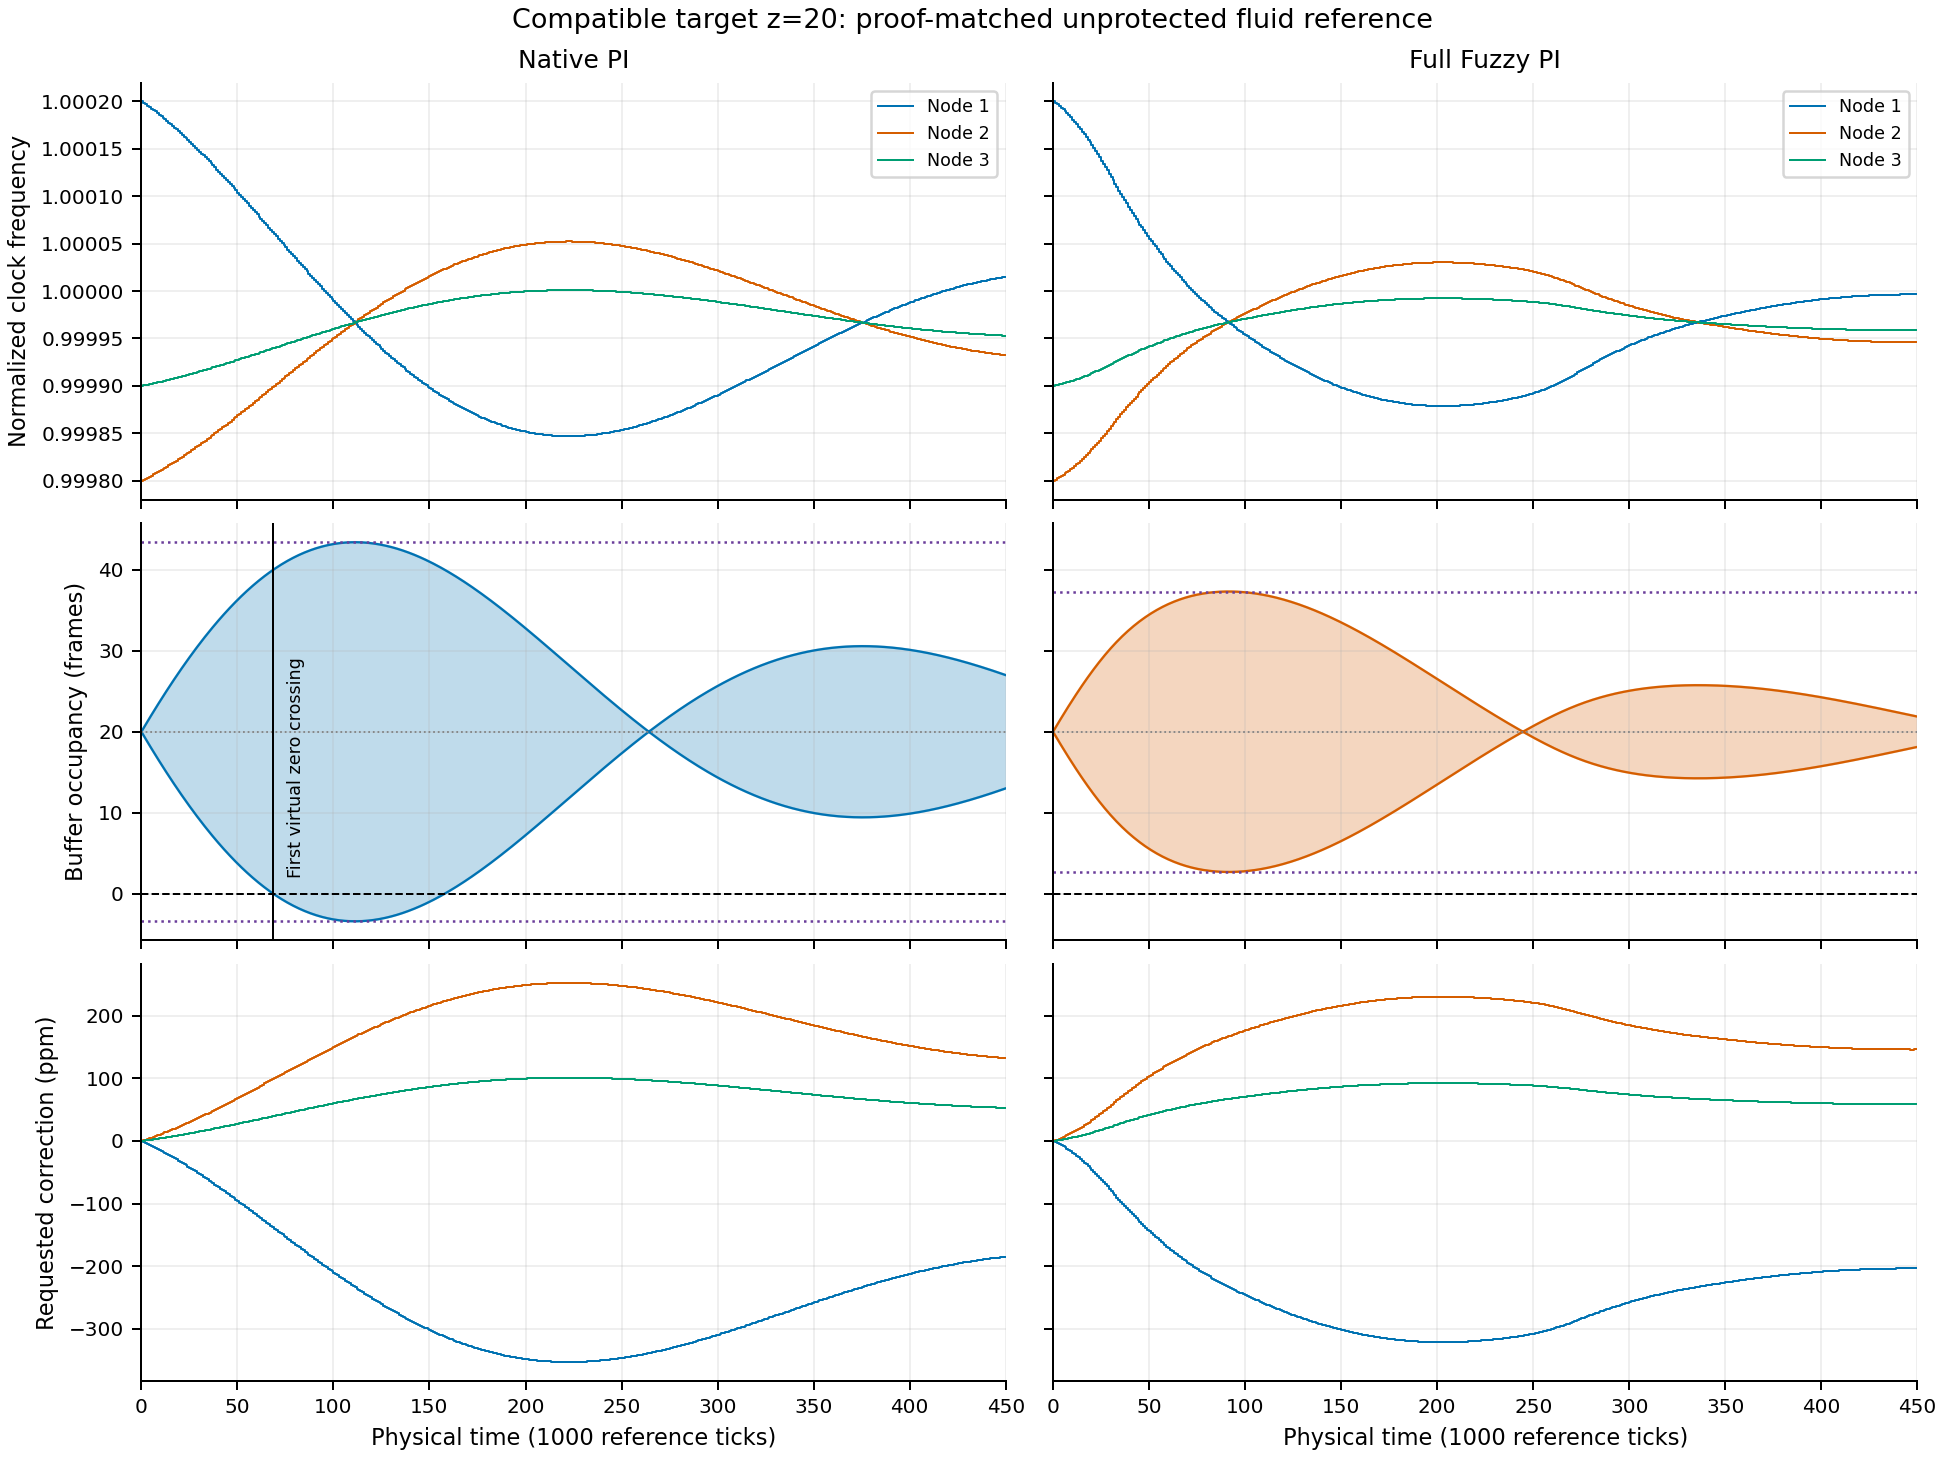
\includegraphics[width=0.94\textwidth]{images/safety_validation_20261105/reference_z20.png}
 \caption{Proof-matched continuous fluid reference at $z=20$ and 400-ppm
 initial spread. Occupancy bands cover all six channels. Fuzzy remains
 above zero, while the unprotected PI trajectory crosses the lower
 boundary. Dotted bounds come from the separate all-time certificate.
 Applied physical frequencies stay positive; signed corrections may be negative.}
 \Description{Matched PI and Fuzzy clock frequencies, fluid buffer envelopes and correction transients.}
 \label{fig:safety_reference_z20}
\end{figure*}

The mismatch grid is
$s\in\{0.25,\allowbreak0.5,\allowbreak0.75,\allowbreak0.85,\allowbreak0.86,\allowbreak1,\allowbreak1.125,\allowbreak1.25,\allowbreak1.5,\allowbreak2\}$.
Figure~\ref{fig:safety_domain} separates the joint sufficient inner
domain from finite-horizon observations at the frozen grid points.
At $z=20$, PI excursions of 19.893146 and 20.127183 frames at
$s=0.85$ and 0.86 bracket its proved directional capacity threshold.
The Fuzzy excursions are computed directly, not scaled linearly.
Successful sampled points do not certify the regions between them;
failure of a sufficient test is recorded as uncertified.

\begin{figure*}[t]
 \centering
 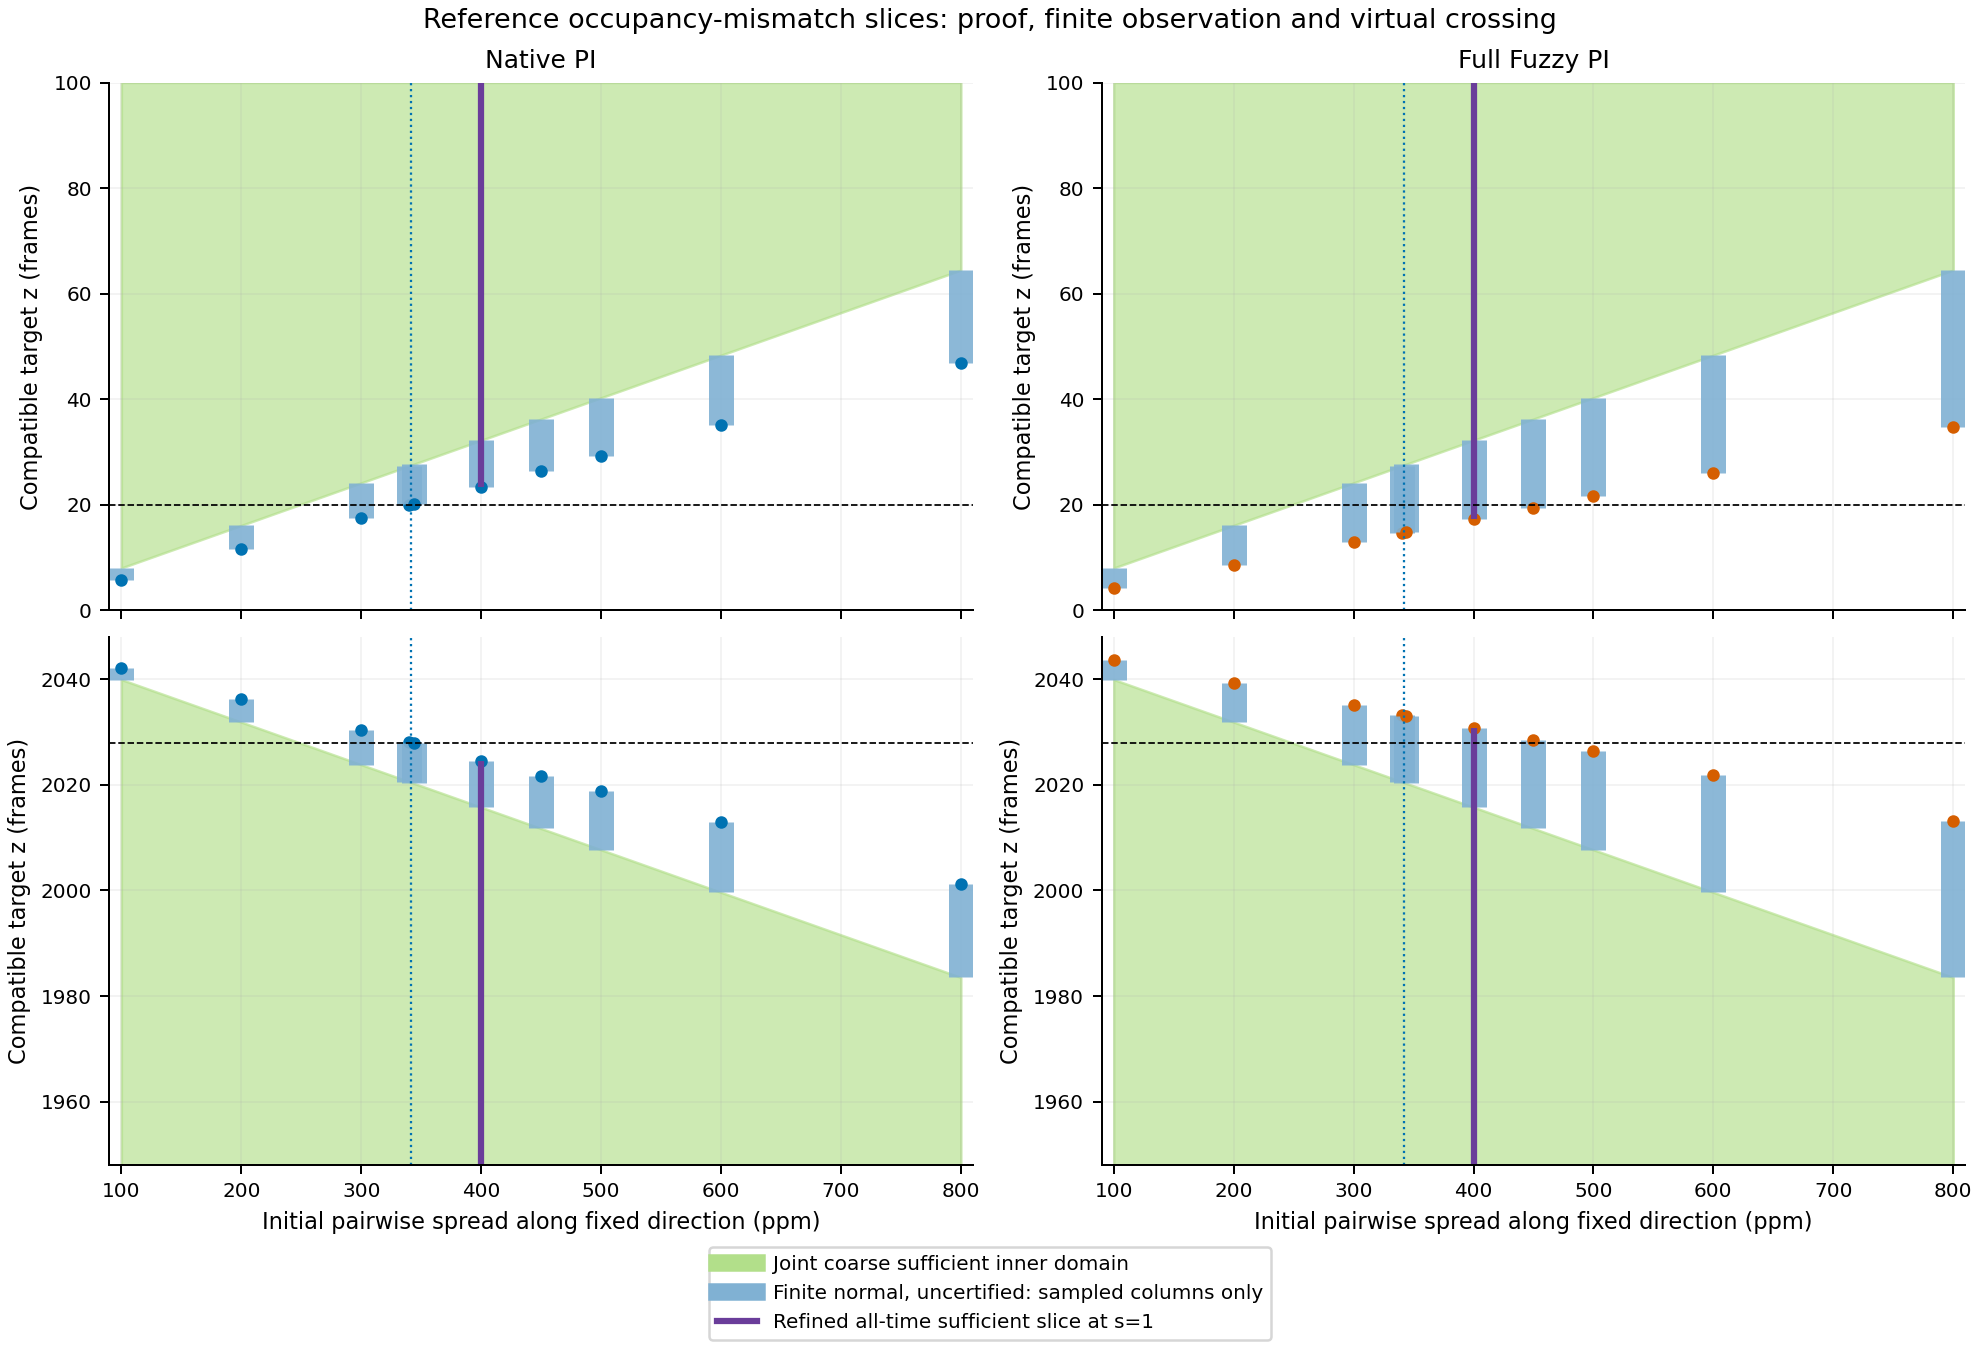
\includegraphics[width=0.94\textwidth]{images/safety_validation_20261105/occupancy_mismatch_domain.png}
 \caption{Compatible-target--mismatch slices at fixed capacity and gains.
 Green denotes the joint coarse sufficient domain. Blue columns extend
 to finite-horizon normal observations at sampled spreads only; markers
 give observed excursion boundaries. Purple denotes the sharper all-time
 slice at $s=1$. The dotted line is PI's directional threshold at $z=20$.
 Central targets are omitted for readability. No untested interpolation
 or delayed-Callisto safety boundary is asserted.}
 \Description{Reference safe configuration slices separating sufficient certificates from sampled trajectory evidence.}
 \label{fig:safety_domain}
\end{figure*}

For the uniform annex, an independent recomputation checks every
one of the 20 parameter cells and reproduces the all-time bound
below 17.342 over 399.6--400.4 ppm. Four direct endpoint runs
are consistent: Fuzzy minima are 2.703366 and 2.668520, whereas
PI minima are $-3.380298$ and $-3.427105$. Their role is to check
the implementation and endpoints; full cell coverage and the
contracting tail supply the uniform theorem.

Two additional zero-mean frequency directions complete the
distribution check. Together with the prescribed direction, all
have 400-ppm spread but $Q=(216,234,288)/30000^2$. Each satisfies
the exact $V_1=H^2c_PQ$ relation. Their Fuzzy peaks differ
(approximately 17.311137, 17.314057 and 17.322842 frames), while
PI peaks coincide for these triangle cases. The energy relation
is a sufficient-domain tool, not an exact-peak ordering rule.

\subsection{Delayed Callisto: normal operation versus protection}
The actual startup cases fix $s=4$, or 1600-ppm initial spread, and
$z\in\{64,83,104,1944,1965,1984\}$. These assess whether the
margin mechanism persists with local timing and integer frames;
they do not apply the reference's numerical boundary to a different
execution model. The low-target cases produce the predicted
qualitative separation (Table~\ref{tab:safety_actual_lower}). At
$z=83$, Fuzzy stays in $[11,155]$ without intervention, while PI
reaches zero and invokes five input-empty guard episodes. The first
occurs at about $71844.672$ physical ticks; summed blocked time is
61.0114 node-ticks. Figure~\ref{fig:safety_actual_z83} distinguishes
physical clock motion from guarded data progress. At $z=64$ both
methods need protection; at $z=104$ both remain normal.
The advantage is therefore positive reserve without pausing the data
execution at the same configuration. PI's guard prevents an invalid
read; the observation is not a physical negative-buffer failure.

\begin{table}[t]
 \caption{Actual low-target startup at matched gains. Ranges include
 every integer event; guard counts are off episodes, not off/on transitions.}
 \label{tab:safety_actual_lower}
 \centering
 \begin{tabular}{@{}rllll@{}}\toprule
 & \multicolumn{2}{c}{Buffer occupancy / frames} & \multicolumn{2}{c}{Guard episodes}\\
 $z$ & PI & Fuzzy & PI & Fuzzy\\\midrule
 64 & 0--128 & 0--128 & 26 & 6\\
 83 & 0--166 & 11--155 & 5 & 0\\
 104 & 10--198 & 32--176 & 0 & 0\\\bottomrule
 \end{tabular}
\end{table}

\begin{figure*}[t]
 \centering
 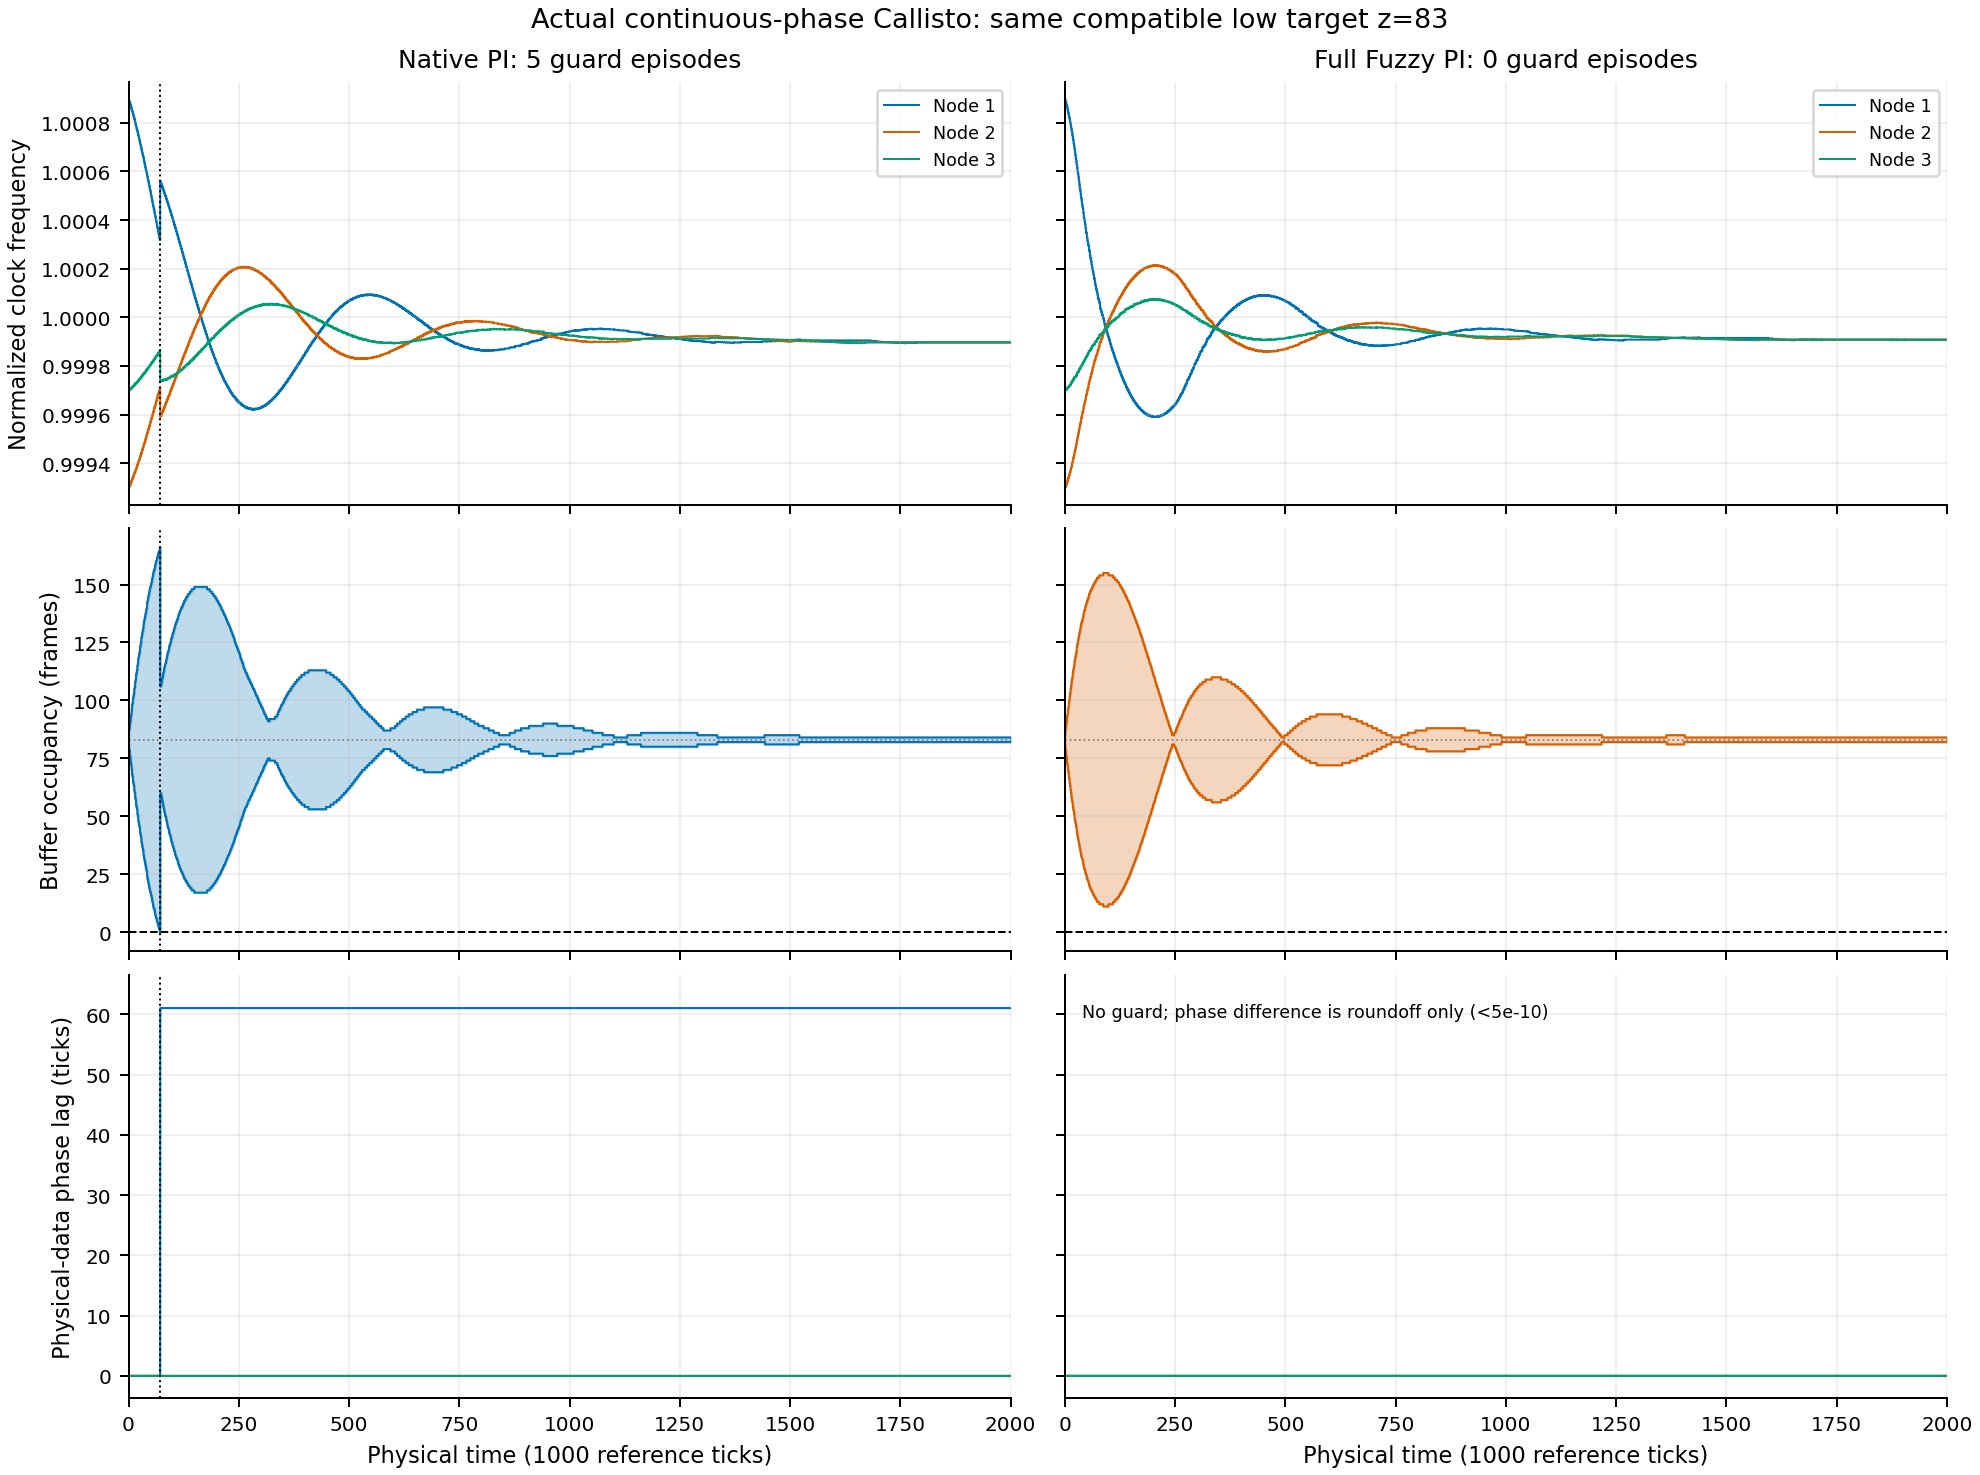
\includegraphics[width=0.94\textwidth]{images/safety_validation_20261105/actual_z83.png}
 \caption{Continuous-phase Callisto at $z=83$, 1600-ppm spread and matched
 gains. Full-event occupancy envelopes show PI reaching zero and Fuzzy
 retaining positive reserve. The dotted line marks PI's first guard.
 Physical-minus-data phase reveals guard-induced progress loss; both
 columns use common axis ranges. This finite delayed execution supports
 the mechanism and is separate from the zero-delay all-time proof.}
 \Description{Actual clock frequencies, buffer occupancies and physical-to-data phase lag for PI and Fuzzy.}
 \label{fig:safety_actual_z83}
\end{figure*}

The upper-target results expose an additional configuration
constraint. All six upper-target runs invoke outgoing-credit
guards even though their maximum receiving occupancy is 2008,
below $\beta_{\max}=2048$. Equation~\eqref{eq:fpi_credit_decomposition}
explains the additional constraint: initial forward-transit and
unacknowledged-consumption counts are both 20, so used credit
starts at $z+40$, rather than at receiving occupancy $z$.
Thus a simple physical-occupancy mirror of the zero-delay result
does not predict guard-free delayed execution. This configuration-
specific 40-frame observation is not a general latency margin.

All 12 runs retain inclusive physical capacity compliance and
positive clock frequency (minimum 0.9993), without correction
saturation. Nine cases rely on guards. Complete crossing replay
has zero occupancy mismatches, and independent command
reconstruction has maximum residual $1.09\times10^{-19}$.
Pre-first-guard command and measurement prefixes match the old
high-reserve trajectory exactly; all post-guard evolution is newly
run. Fewer guard episodes alone does not prove higher throughput:
at $z=1965$ Fuzzy has fewer episodes but lower final data progress.
Appendix~\ref{app:safety_validation} retains every case, credit
diagnostics and the complete validation protocol.

\subsection{Supplementary disturbance-performance evidence}
Earlier independent tuning and random/burst campaigns answer a
different question. Their complete protocols and results, including
operating limits, are retained in Appendix~\ref{app:evaluation}.
They are not rerun or used as evidence for the safety-domain theorem.
The present evidence chain is the mathematical configuration test,
strict reference comparison and qualitative implementation checks.
